\documentclass[12pt]{article}
\usepackage{latexblog}

% ============================================================
% Blog Metadata
% ============================================================
\blogtitle{递归和迭代}
\blogdate{2021-02-26}
\blogtags{编程语言, Scheme, 闲话编程}
\bloglang{zh}
\blogsummary{}

\begin{document}
\makeblogtitle

这是读《计算机程序的构造和解释》的笔记。

\section{递归和迭代}\label{ux9012ux5f52ux548cux8fedux4ee3}

\subsection{计算裴波拉切数列}\label{ux8ba1ux7b97ux88f4ux6ce2ux62c9ux5207ux6570ux5217}

裴波拉切数列是很简单的过程，其数学公式如下：

\[
Fib(n)=\left\{
\begin{array}{rcl}
0 & {n = 0}\\
1 & {n = 1}\\
Fib(n-1) + Fib(n-2) & {n > 1}\\
\end{array} \right.
\]

使用递归非常容易解决，就是直接将这个公式翻译成计算机语言即可：

\begin{Shaded}
\begin{Highlighting}[]
\NormalTok{(}\ExtensionTok{define}\FunctionTok{ }\NormalTok{(}\FunctionTok{fib }\NormalTok{n)}
\NormalTok{    (}\KeywordTok{cond} 
\NormalTok{        ((}\OperatorTok{=}\NormalTok{ n }\DecValTok{0}\NormalTok{) }\DecValTok{0}\NormalTok{)}
\NormalTok{        ((}\OperatorTok{=}\NormalTok{ n }\DecValTok{1}\NormalTok{) }\DecValTok{1}\NormalTok{)}
\NormalTok{        (}\KeywordTok{else}\NormalTok{ (}\OperatorTok{+}\NormalTok{ (fib (}\OperatorTok{{-}}\NormalTok{ n }\DecValTok{1}\NormalTok{))}
\NormalTok{                 (fib (}\OperatorTok{{-}}\NormalTok{ n }\DecValTok{2}\NormalTok{)))}
\NormalTok{        )}
\NormalTok{    )}
\NormalTok{)}
\end{Highlighting}
\end{Shaded}

这个递归算法虽然实现很简单，但却有比较大的性能问题，出现了不必要的计算。例如计算Fib(5)，其计算过程如下：

\begin{figure}
\centering
\pandocbounded{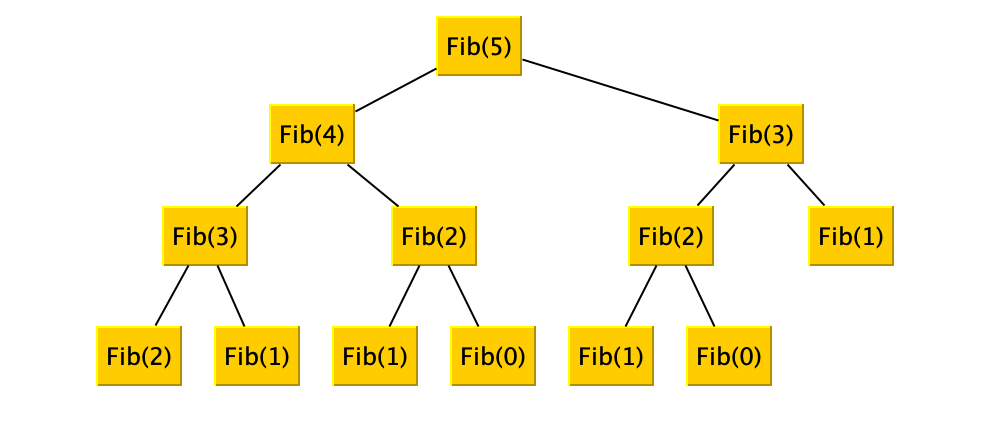
\includegraphics[keepaspectratio,alt={Fib(5)}]{images/Fib-tree.png}}
\caption{Fib(5)}
\end{figure}

其中Fib(2)就计算了三次。那么，如何使用迭代来计算呢？迭代的思想在于给定若干变量的初始值，不断根据规则进行计算来改变这些变量，最后进行N次之后得到最终的结果。

\[
\begin{cases}
a = Fib(1) \\
b = Fib(0)
\end{cases}
\xrightarrow[\text{进行迭代}]{}
\begin{cases}
a = a + b \\
b = a
\end{cases}
\xrightarrow[\text{通过n次迭代变成}]{}
\begin{cases}
a = Fib(n+1)) \\
b = Fib(n)
\end{cases}
\]

这样实际上需要三个变量：

\[
\begin{cases}
F_{n} \\
F_{n+1} \\
Count
\end{cases}
\xrightarrow[\text{初始值}]{}
\begin{cases}
F_{n} &= Fib(0)\\
F_{n+1} &= Fib(1) \\
Count &= n
\end{cases}
\xrightarrow[\text{第一次迭代}]{}
\begin{cases}
F_{n} &= Fib(1)\\
F_{n+1} &= Fib(0) + Fib(1) \\
Count &= n - 1
\end{cases}\\
\xrightarrow[\text{第n次迭代}]{}
\begin{cases}
F_{n} &= Fib(n)\\
F_{n+1} &= Fib(n-1) + Fib(n) \\
Count &= 0
\end{cases}
\]

那么，翻译成代码就是：

\begin{Shaded}
\begin{Highlighting}[]
\NormalTok{(}\ExtensionTok{define}\FunctionTok{ }\NormalTok{(}\FunctionTok{fib }\NormalTok{n)}
\NormalTok{     (fib\_iter }\DecValTok{1} \DecValTok{0}\NormalTok{ n)}
\NormalTok{)}

\NormalTok{(}\ExtensionTok{define}\FunctionTok{ }\NormalTok{(}\FunctionTok{fib\_iter }\NormalTok{a b i)}
\NormalTok{    (}\KeywordTok{if}\NormalTok{ (}\OperatorTok{=}\NormalTok{ i }\DecValTok{0}\NormalTok{)}
\NormalTok{        b}
\NormalTok{        (fib\_iter (}\OperatorTok{+}\NormalTok{ a b) a (}\OperatorTok{{-}}\NormalTok{ i }\DecValTok{1}\NormalTok{))}
\NormalTok{    )}
\NormalTok{)}
\end{Highlighting}
\end{Shaded}


\end{document}
